\begin{name}
	{\tenchude}
	{TOÁN 10}
	{LỚP TOÁN THẦY PHÁT}
	{Thời gian: 90 phút - Không kể thời gian phát đề}
\end{name}
\TN
\Opensolutionfile{ans}[ans/ansBONPA-0D1-OnChuong-De2]
\begin{ex}%Câu 1%[0D1H2-1]
	Số phần tử của tập hợp $A=\left\{{k^2}+1\big|k\in\mathbb{Z},\left| k\right|\le 2\right\}$ là
	\choice
	{$1$}
	{$2$}
	{\True $3$}
	{$5$}
	\loigiai{
		$A=\left\{{k^2}+1\left| k\in\mathbb{Z},\left| k\right|\le 2\right.\right\}$. Ta có $k\in\mathbb{Z}$, $\left| k\right|\le 2$ $\Leftrightarrow-2\le k\le 2$ $\Rightarrow A=\left\{ 1;\,2;\,5\right\}.$.}
\end{ex}

\begin{ex}%Câu 2%[0D1H2-1]
	Tập $A=\left\{ x\in\mathbb{R}\left|-3<1-2x\le 1\right.\right\}$ được viết lại dưới dạng đoạn, khoảng, nửa khoảng là
	\choice
	{$\left(-1;\,0\right]$}
	{\True $\left[0;\,2\right)$}
	{$\left[1;\,2\right]$}
	{$\left(0;\,2\right]$}
	\loigiai{
		Ta có $-3<1-2x\le 1\Leftrightarrow-4<-2x\le 0\Leftrightarrow 0\le x<2$.\\
		Do đó $A=\left\{ x\in\mathbb{R}\left| 0\le x<2\right.\right\}=\left[0;\,2\right)$.}
\end{ex}

\begin{ex}%Câu 3%[0D1N1-5]
	Trong các mệnh đề sau, mệnh đề nào \textbf{sai}?
	\choice
	{$\exists x\in\mathbb{R}\colon x^2-3x+2=0$}
	{$\forall x\in\mathbb{R}\colon x^2\ge 0$}
	{$\exists n\in\mathbb{N}\colon n^2=n$}
	{\True $\forall n\in\mathbb{N}$ thì $n<2n$}
	\loigiai{
		Xét mệnh đề \lq\lq$\forall n\in\mathbb{N}$ thì $n<2n$\rq\rq.\\
		Chọn $n=0\in\mathbb{N}\Rightarrow 2n=0\Rightarrow n=2n$\\
		$\Rightarrow \forall n\in\mathbb{N}$ thì $n<2n$ là mệnh đề sai.}
\end{ex}

\begin{ex}%Câu 4%[0D1N1-5]
	Tìm mệnh đề đúng?
	\choice
	{$\lq\lq\exists x\in\mathbb{R}\colon{x^2}+3=0$\rq\rq}
	{\lq\lq$\forall x\in\mathbb{Z}\colon{x^5}>x^2$\rq\rq}
	{\True \lq\lq$\forall x\in\mathbb{N}\colon\left(2x+1\right)^2-1$ chia hết cho $4$\rq\rq}
	{\lq\lq$\exists x\in\mathbb{R}\colon{x^4}+3x^2+2=0$\rq\rq}
	\loigiai{
		Ta có $\left(2x+1\right)^2-1=4x^2+4x+1-1=4x\left(x+1\right).$\\
		Vì $4\,\vdots\, 4$ nên $4x\left(x+1\right)\,\vdots\, 4$, $\forall x\in\mathbb{N}$.\\
		Suy ra tồn tại số thực $\hoac{
			& x>1\\ 
			& x<0}$ thỏa mãn $x^2>x$.}
\end{ex}
%
\begin{ex}%Câu 5%[0D1N2-1]
	Hãy liệt kê các phần tử của tập hợp $X=\left\{ x\in\mathbb{R}\big|{x^4}-6x^2+8=0\right\}$.
	\choice
	{$X=\left\{ 2;4\right\}$}
	{$X=\left\{-\sqrt{2};\sqrt{2}\right\}$}
	{$X=\left\{\sqrt{2};2\right\}$} {$X=\left\{-\sqrt{2};\sqrt{2};-2;2\right\}$}
	\loigiai{
		Giải phương trình $x^4-6x^2+8=0\Leftrightarrow\hoac{
			&x^2=2\\ 
			&x^2=4}\Leftrightarrow\hoac{
			& x=\pm\sqrt{2}\\ 
			& x=\pm 2.}$}\\
	Vậy $X=\left\{-\sqrt{2};\sqrt{2};-2;2\right\}$.
\end{ex}

\begin{ex}%Câu 6%[0D1H2-1]
	Trong các tập hợp sau, tập hợp nào là tập rỗng?
	\choice
	{$A=\left\lbrace  x\in\mathbb{N}\big|x^2-4=0\right\rbrace $}
	{\True $B=\left\lbrace x\in\mathbb{R}\big|x^2+2x+3=0\right\rbrace $}
	{$C=\left\lbrace  x\in\mathbb{R}\big|x^2-5=0\right\rbrace $}
	{$D=\left\lbrace  x\in\mathbb{Q}\big|x^2+x-12=0\right\rbrace $}
	\loigiai{
		$A=\left\lbrace  x\in\mathbb{N}\big|x^2-4=0\right\rbrace \Rightarrow A=\left\{2\right\}$.\\
		$B=\left\{ x\in\mathbb{R}\big|x^2+2x+3=0\right\}\Rightarrow B=\varnothing .$\\
		$C=\left\{ x\in\mathbb{R}\big|x^2-5=0\right\}\Rightarrow C=\left\{-\sqrt{5};\sqrt{5}\right\}.$\\
		$D=\left\{ x\in\mathbb{Q}\big|x^2+x-12=0\right\}\Rightarrow D=\left\{-3;\,4\right\}$.
	}
\end{ex}
%
\begin{ex}%Câu 7%[0D1H2-2]
	Cho tập hợp $A=\left\{ 1;2;5;7\right\}$ và $B=\left\{ 1;2;3\right\}$. Có tất cả bao nhiêu tập $X$ thỏa mãn $X\subset A$ và $X\subset B$?
	\choice
	{$2$}
	{\True $4$}
	{$6$}
	{$8$}
	\loigiai{
		Vì $\heva{
			& X\subset A\\ 
			& X\subset B}$ nên $X\subset\left(A\cap B\right)$.\\
		Mà $A\cap B=\left\{ 1;2\right\}$. Nên có $2^2=4$ tập $X$.
	}
\end{ex}
%
\begin{ex}%Câu 8%[0D1N2-3]
	Hình vẽ nào sau đây (phần không bị gạch) minh họa cho tập hợp $\left(1;4\right]$?
	\choice
	{\True 		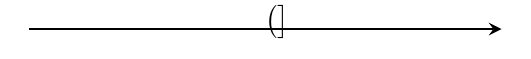
\begin{tikzpicture}[>=stealth,line width=1pt]
			\draw[->](-3,0)->(3,0);		%Vẽ trục số
			\def\skipInterval{0.5cm}		%Khoảng cách đặt nhãn
			%\def\colorInterval{blue} 	%Màu tick, màu fill miền
			%\IntervalR{\big(}{1}{\big]}{4}
			\IntervalLR{-3}{-1.4}		\IntervalGLF{}{}{\big(}{1}
			\IntervalLR{3}{1}	
			\IntervalGLF{}{}{\big]}{4}
		\end{tikzpicture}
	}
	{	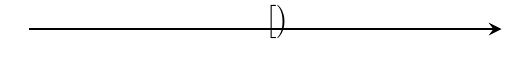
\begin{tikzpicture}[>=stealth,line width=1pt]
			\draw[->](-3,0)->(3,0);		%Vẽ trục số
			\def\skipInterval{0.5cm}		%Khoảng cách đặt nhãn
			%\def\colorInterval{blue} 	%Màu tick, màu fill miền
			%\IntervalR{\big(}{1}{\big]}{4}
			\IntervalLR{-3}{-1.4}		\IntervalGLF{}{}{\big[}{1}
			\IntervalLR{3}{1}	
			\IntervalGLF{}{}{\big)}{4}
		\end{tikzpicture}
	}
	{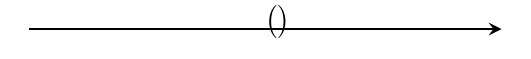
\begin{tikzpicture}[>=stealth,line width=1pt]
			\draw[->](-3,0)->(3,0);		%Vẽ trục số
			\def\skipInterval{0.5cm}		%Khoảng cách đặt nhãn
			%\def\colorInterval{blue} 	%Màu tick, màu fill miền
			%\IntervalR{\big(}{1}{\big]}{4}
			\IntervalLR{-3}{-1.4}		\IntervalGLF{}{}{\big(}{1}
			\IntervalLR{3}{1}	
			\IntervalGLF{}{}{\big)}{4}
		\end{tikzpicture}
	}
	{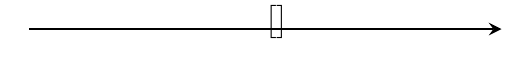
\begin{tikzpicture}[>=stealth,line width=1pt]
			\draw[->](-3,0)->(3,0);		%Vẽ trục số
			\def\skipInterval{0.5cm}		%Khoảng cách đặt nhãn
			%\def\colorInterval{blue} 	%Màu tick, màu fill miền
			%\IntervalR{\big(}{1}{\big]}{4}
			\IntervalLR{-3}{-1.4}		\IntervalGLF{}{}{\big[}{1}
			\IntervalLR{3}{1}	
			\IntervalGLF{}{}{\big]}{4}
		\end{tikzpicture}
	}
	\loigiai{
		Vì $\left(1;4\right]$ gồm các số thực $x$ mà $1<x\le 4$ nên biểu diễn trên trục là\begin{center} 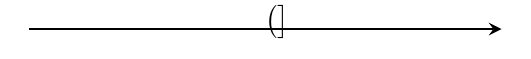
\begin{tikzpicture}[>=stealth,line width=1pt]
				\draw[->](-3,0)->(3,0);		%Vẽ trục số
				\def\skipInterval{0.5cm}		%Khoảng cách đặt nhãn
				%\def\colorInterval{blue} 	%Màu tick, màu fill miền
				%\IntervalR{\big(}{1}{\big]}{4}
				\IntervalLR{-3}{-1.4}		\IntervalGLF{}{}{\big(}{1}
				\IntervalLR{3}{1}	
				\IntervalGLF{}{}{\big]}{4}
	\end{tikzpicture}\end{center}}
\end{ex}
%
\begin{ex}%Câu 9%[0D1N2-1]
	Cho tập hợp $A=\left\{1,2,3,4,x,y\right\}$. Xét các mệnh đề sau đây:\\
	$(I)$: \lq\lq$3\in A$\rq\rq.\\
	$\left(II\right)$: \lq\lq$\left\{ 3,4\right\}\in A$\rq\rq.\\
	$\left(III\right)$: \lq\lq$\left\{ a,3,b\right\}\in A$\rq\rq.\\
	Trong các mệnh đề sau, mệnh đề nào đúng?
	\choice
	{\True $I$ đúng}
	{$I$, $II$ đúng}
	{$II$, $III$ đúng}
	{$I$, $III$ đúng}
	\loigiai{
		$3$ là một phần tử của tập hợp $A$.\\
		$\left\{ 3,4\right\}$ là một tập con của tập hợp $A$. Ký hiệu $\left\{ 3,4\right\}\subset A$.\\
		$\left\{ a,3,b\right\}$ là một tập con của tập hợp $A$. Ký hiệu $\left\{ a,3,b\right\}\subset A$.}
\end{ex}
%
\begin{ex}%Câu 10%[0D1H2-2]
	Có tất cả bao nhiêu tập $X$ thỏa mãn $\left\{ 1;2;3\right\}\subset X\subset\left\{ 1;2;3;4;5;6\right\}$?
	\choice
	{$1$}
	{\True $8$}
	{$3$}
	{$6$}
	\loigiai{
		Các tập hợp $X$ thỏa mãn điều kiện là\allowdisplaybreaks
		\begin{eqnarray*}
			X&=&\left\{ 1;2;3\right\}, X=\left\{ 1;2;3;4\right\},\\
			X&=&\left\{ 1;2;3;5\right\}, X=\left\{ 1;2;3;6\right\},\\
			X&=&\left\{ 1;2;3;4;5\right\}, X=\left\{ 1;2;3;4;6\right\},\\
			X&=&\left\{ 1;2;3;5;6\right\}, X=\left\{ 1;2;3;4;5;6\right\}.
		\end{eqnarray*}
		Vậy có tất cả $8$ tập hợp $X$ thỏa mãn yêu cầu bài toán.}
\end{ex}
%
\begin{ex}%Câu 11%[0D1H3-5]
	Lớp 10A có $10$ học sinh giỏi Toán, $10$ học sinh giỏi Lý, $11$ học sinh giỏi hóa, $6$ học sinh giỏi cả Toán và Lý, $5$ học sinh giỏi cả Hóa và Lý, $4$ học sinh giỏi cả Toán và Hóa, $3$ học sinh giỏi cả ba môn Toán, Lý, Hóa). Số học sinh giỏi ít nhất một trong ba môn (Toán, Lý, Hóa) của lớp 10A là
	\choice
	{\True $19$}
	{$18$}
	{$31$}
	{$49$}
	\loigiai{Gọi $T$ là tập hợp học sinh giỏi toán, $L$ là tập hợp học sinh giỏi lý, $H$ là tập hợp học sinh giỏi hóa.\\
		Theo giả thiết ta có\allowdisplaybreaks
		\begin{eqnarray*}
			&&|T|=10; |L|=10; |H|=11;\\
			&&|T\cap L|=6; |T\cap H|=4; |L\cap H|=5;\\
			&& |T\cap L\cap H|=3.
		\end{eqnarray*}
		Số học sinh giỏi ít nhất một trong ba môn (Toán, Lý, Hóa) của lớp 10A là
		$$|T\cup L\cup H|=|T|+|L|+|H|-|T\cap L|-|T\cap H|-|L\cap H|+|T\cap L\cap H|=10+10+11-6-4-5+3=19.$$
	}
\end{ex}
%
\begin{ex}%Câu 12%[0D1H3-5]
	Mỗi học sinh của lớp $10A_1$ đều học giỏi môn Toán hoặc môn Hóa, biết rằng có $30$ học sinh giỏi Toán, $35$ học sinh giỏi Hóa, và $20$ em học giỏi cả hai môn. Hỏi lớp $10A_1$ có bao nhiêu học sinh?
	\choice
	{$40$}
	{\True $45$}
	{$50$}
	{$55$}
	\loigiai{Gọi $T$ là tập hợp học sinh giỏi toán, $H$ là tập hợp học sinh giỏi hóa.\\
		Theo giả thiết ta có $|T|=30$; $|H|=35$;  $|T\cap H|=20$.\\
		Sĩ số học sinh lớp $10A_1$ là $|T\cup H|=|T|+|H|-|T\cap H|=30+35-20=45$.}
\end{ex}

\Closesolutionfile{ans}
\TNTF
\setcounter{ex}{0}
\Opensolutionfile{ans}[ans/ansDS-0D1-OnChuong-De2]
%
\begin{ex}%Câu 13%[0D1H1-5]
	Xét tính đúng, sai của mỗi mệnh đề sau.
	\choiceTF
	{\True $\exists x\in\mathbb{Q}, 4 x^2-1=0$}
	{$\forall n\in\mathbb{N}, n$ và $n+2$ là các số nguyên tố}
	{$\forall x\in\mathbb{R},(x-1)^2\neq x-1$}
	{$\forall n\in\mathbb{N}, n^2>n$}
	\loigiai{
		\begin{itemchoice}
			\itemch  Ta có $4 x^2-1=0\Leftrightarrow x=\pm\dfrac{1}{2}\in\mathbb{Q}$.
			\itemch Ta cho $n=2\in\mathbb{N}$ thì $n+2=4$ không là số nguyên tố.
			\itemch Ta cho $x=1\in\mathbb{R}$ thì $(x-1)^2=x-1=0$.
			\itemch  Ta cho $n=0\in\mathbb{N}$ thì $n^2=0$ nên $n^2>n$ là sai.
	\end{itemchoice}}
\end{ex}
%
\begin{ex}%Câu 14%[0D1H1-2]
	Xét tính đúng, sai của mỗi mệnh đề sau.
	\choiceTF
	{\True Hai góc đối đỉnh thì bằng nhau}
	{\True Hai tam giác có hai cặp cạnh bằng nhau và cặp góc xen giữa hai cạnh bằng nhau thì bằng nhau}
	{Hai tam giác có hai cặp góc bằng nhau thì bằng nhau}
	{\True Một số chia hết cho $3$ khi và chỉ khi tổng các chữ số chia hết cho $3$}
	\loigiai{
		\begin{itemchoice}
			\itemch Lý thuyết.
			\itemch Lý thuyết.
			\itemch 
			\itemch Lý thuyết.
		\end{itemchoice}
	}
\end{ex}
%
\begin{ex}%Câu 15%[0D1H3-4]
	Cho các tập hợp $A=\{0 ; 1 ; 2 ; 3 ; 4\}$; $ B=\{0 ; 1 ; 2\}$; $C=\{-3 ; 0 ; 1 ; 2\}$. Khi đó
	\choiceTF
	{\True $A\setminus B=\{3 ; 4\}$}
	{\True $(A\cap C)\setminus B=\varnothing$}
	{$A\cup (C\setminus B)=\{-3;0;1;4\}$}
	{$C_AB=\{1;3;4\}$}
	\loigiai{
		\begin{itemchoice}
			\itemch $A\setminus B=\{3 ; 4\}$.
			\itemch $(A\cap C)\setminus B=\varnothing$.
			\itemch $A\cup(C\setminus B)=\{-3 ; 0 ; 1 ; 2 ; 3 ; 4\}$.
			\itemch $C_A B=\{3 ; 4\}$.
		\end{itemchoice}
	}
\end{ex}
%
\begin{ex}%Câu 16%[0D1H3-4]
	Cho $A$ là tập hợp các học sinh lớp 10 đang học ở trường em và $B$ là tập hợp các học sinh đang học môn Tiếng Anh của trường em. Vậy
	\choiceTF
	{\True $A\cap B$ là tập hợp các học sinh lớp 10 học môn Tiếng Anh ở trường em}
	{\True $A\setminus B$ là tập hợp những học sinh lớp 10 nhưng không học Tiếng Anh ở trường em}
	{\True $A\cup B$ là tập hợp các học sinh lớp 10 hoặc học sinh học môn Tiếng Anh ở trường em}
	{\True $B\setminus A$ là tập hợp các học sinh học môn Tiếng Anh nhưng không học lớp 10 ở trường em}
	\loigiai{
		\begin{itemchoice}
			\itemch $A\cap B$ là tập hợp các học sinh lớp $10$ học môn Tiếng Anh ở trường em.
			\itemch $A\setminus B$ là tập hợp những học sinh lớp $10$ nhưng không học Tiếng Anh ở trường em.
			\itemch $A\cup B$ là tập hợp các học sinh lớp $10$ hoặc học sinh học môn Tiếng Anh ở trường em.
			\itemch $B\setminus A$ là tập hợp các học sinh học môn Tiếng Anh nhưng không học lớp $10$ ở trường em.
		\end{itemchoice}
	}
\end{ex}

\Closesolutionfile{ans}
\TNSA
\setcounter{ex}{0}
\Opensolutionfile{ans}[ans/ansTLN-0D1-OnChuong-De2]
%
\begin{ex}%Câu 22%[0D1H3-5]
	Một lớp học có $25$ học sinh chơi bóng đá, $23$ học sinh chơi bóng bàn, $14$ học sinh chơi cả bóng đá và bóng bàn, $6$ học sinh không chơi môn thể thao nào. Tìm số học sinh của lớp?\shortans{40}
	\loigiai{
		Gọi $A$ là tập hợp các học sinh chơi bóng đá, $B$ là tập hợp các học sinh chơi bóng bàn,
		$C$ là tập hợp các học sinh không chơi môn thể thao nào.\\
		Ta có $|A|=25$; $|B|=23$; $|C|=6$; $|A\cap B|=14$.\\
		Khi đó số học sinh chỉ chơi một môn thể thao là $|A|+|B|-|A\cap B|+|C|=25+23-14+6=40$.}
\end{ex}
%
\begin{ex}%Câu 7%[0D1H2-2]
	Cho tập hợp $A=\left\{ 1;2;5;7\right\}$ và $B=\left\{ 1;2;3;5\right\}$. Có tất cả bao nhiêu tập $X$ thỏa mãn $X\subset A$ và $X\subset B$ ?
	\shortans{8}
	\loigiai{
		Vì $\left\{\begin{aligned}
			& X\subset A\\ 
			& X\subset B\\ 
		\end{aligned}\right.$ nên $X\subset\left(A\cap B\right)$.\\
		Mà $A\cap B=\left\{ 1;2;5\right\}$. Nên có $2^3=8$ tập $X$.
	}
\end{ex}
%
\begin{ex}%Câu 19%[0D1V3-3]
	Cho hai tập hợp $A=[-4 ; 1], B=[-3 ; m]$. Có bao nhiêu giá trị nguyên của tham số $m$ để $A\cup B=A$?
	\shortans{4}
	\loigiai{
		Điều kiện $m>-3$.\\
		Ta có $A\cup B=A$ khi và chỉ khi $B\subset A$, tức là $m\leqslant 1$.\\
		Đối chiếu điều kiện, ta được $-3<m\leqslant 1$. Suy ra có $4$ giá trị nguyên của tham số $m$.}
\end{ex}
%
\begin{ex}%Câu 20%[0D1H3-4]
	Cho $A$ là tập hợp tất cả các nghiệm của phương trình $x^2-4 x+3=0$;
	$B$ là tập hợp các số nguyên có giá trị tuyệt đối nhỏ hơn $4$. Số phần tử của tập hợp $A\setminus B$ là
	\shortans{0}
	\loigiai{
		Ta có $x^2-7 x+6=0\Leftrightarrow\heva{&x=1\\ &x=3}\Rightarrow A=\{1 ; 3\}$.\\
		$B=\{-3 ;-2 ;-1 ; 0 ; 1 ; 2 ; 3\}$. Do đó $A\setminus B=\varnothing$.}
\end{ex}
%
\begin{ex}%Câu 21%[0D1H3-5]
	Lớp 10A có $45$ học sinh trong đó có 25 em học giỏi môn Toán, $23$ em học giỏi môn Lý, $20$ em học giỏi môn Hóa, $11$ em học giỏi cả môn Toán và môn Lý, $8$ em học giỏi cả môn Lý và môn Hóa, $9$ em học giỏi cả môn Toán và môn Hóa. Hỏi lớp 10A có bao nhiêu bạn học giỏi cả ba môn Toán, Lý, Hóa? (biết rằng mỗi học sinh trong lớp học giỏi ít nhất một trong ba môn Toán, Lý, Hóa).\shortans{5}
	\loigiai{
		Gọi $T$, $L$, $H$ lần lượt là tập hợp các học sinh giỏi môn Toán, Lý, Hóa.\\
		Ta có\allowdisplaybreaks \begin{eqnarray*}
			&&|T\cup L\cup H|=|T|+|L|+|H|-|T\cap L|-|L\cap H|-|H\cap T|+|T\cap L\cap H|\\
			&\Leftrightarrow& 45=25+23+20-11-8-9+|T\cap L\cap H|\\
			&\Leftrightarrow&|T\cap L\cap H|=5.
		\end{eqnarray*}
		Vậy có $5$ học sinh giỏi cả $3$ môn.}
\end{ex}
%
\begin{ex}%Câu 22%[0D1H3-5]
	Một lớp học có $25$ học sinh chơi bóng đá, $23$ học sinh chơi bóng bàn, $14$ học sinh chơi cả bóng đá và bóng bàn. Tìm số học sinh chỉ chơi một môn thể thao?\shortans{20}
	\loigiai{
		Gọi $A$ là tập hợp các học sinh chơi bóng đá, $B$ là tập hợp các học sinh chơi bóng bàn.\\
		Ta có $|A|=25$; $|B|=23$; $|A\cap B|=14$.\\
		Khi đó số học sinh chỉ chơi một môn thể thao là $|A|+|B|-2|A\cap B|=25+23-2\cdot14=20$.}
\end{ex}
\Closesolutionfile{ans}
% \begin{center}	
% 	\fontfamily{qag}\selectfont\color{violet} 	\centering{\textbf{BẢNG ĐÁP ÁN}}
% \end{center}
% \inputansbox{12}{ans/ansBONPA-0D1-OnChuong-De2}
% \inputansbox{4}{ans/ansDS-0D1-OnChuong-De2}
% \inputansbox{6}{ans/ansTLN-0D1-OnChuong-De2}